\chapter[Integrationsprozesse]{Integrationsprozesse}

Nach den behandelten Herausforderungen werden in diesem Kapitel Möglichkeiten und Vorgehensmodelle zur Integration von Data Science in Organisationen thematisiert.
Dazu werden insgesamt drei Modelle der Forschungsliteratur dargelegt.

\section{CSPG Framework}

\Citeauthor*{Grossman.2014} veröffentlichte 2014 das CSPG Framework zur Integration von Analytik, Domänenwissen und IT in Organisationen.
\textit{CSPG} steht dabei repräsentativ als Abkürzung für die Komponenten \textit{Culture, Staffing, Processes} und \textit{Governance}. 
Der Aspekt der Kultur ist dabei durch die Organisationsleitung umzusetzen, indem Verantwortung und Authorität für Datenbestände an eine Funktionsstelle übergeben wird.
Die Aufnahme von Data Science Personal ist im CSPG Framework unausweichlich und durch den Analytikleiter und die Geschäftsleitung durchzuführen. 
Dabei ist zu entscheiden, ob die analytische Funktion zentral, dezentral oder hybrid organisiert wird.
Im dritten Aspekt des Frameworks sind die analytischen Prozesse in der Organisation aufzubauen.
Ein Teil dieser Prozesse umfasst den Austausch von Daten zwischen Abteilungen und anderen Organisationen.
Weitere Prozesse behandeln die Digitalisierung bestehender Inhalte, Produktanpassung zur Aufnahme von Daten und die Kombination von Datenbeständen mit anderen Industrien.
Die finale Komponente des Frameworks ist der Aufbau, die Verwaltung und die Weiterentwicklung der notwendigen Infrastruktur.
Zur Bewältigung dieser Aufgabe sind die folgenden vier Parameter in der Organisation einzustellen:

\begin{itemize}
    \item Langfristige Verpflichtung für Data Science und Sicherstellung des daraus entstehenden Geschäftswerts.
    \item Sichere und rechtlich unbedenkliche Umsetzung der Data Science Prozesse.
    \item Herstellen von Haftbarkeit, Transparenz und Rückverfolgbarkeit für Projektfinanzierung, Entwicklung und Ressourcen.
    \item Ressourcenbereitstellung für Daten-, Analyse- und Managementprozesse.
\end{itemize}

\section{Design Parameters}

Durch die Arbeit von \Citeauthor*{JanineAdinaHagen.2020} konnten die Gestaltungsparameter einer datengesteuerten Organisation ermittelt werden.
Diese Parameter können als Anleitung betrachtet werden, wie die eigene Organisation in verschiedenen Aspekten zu gestalten ist.

\begin{figure}[htb]
    \centering
    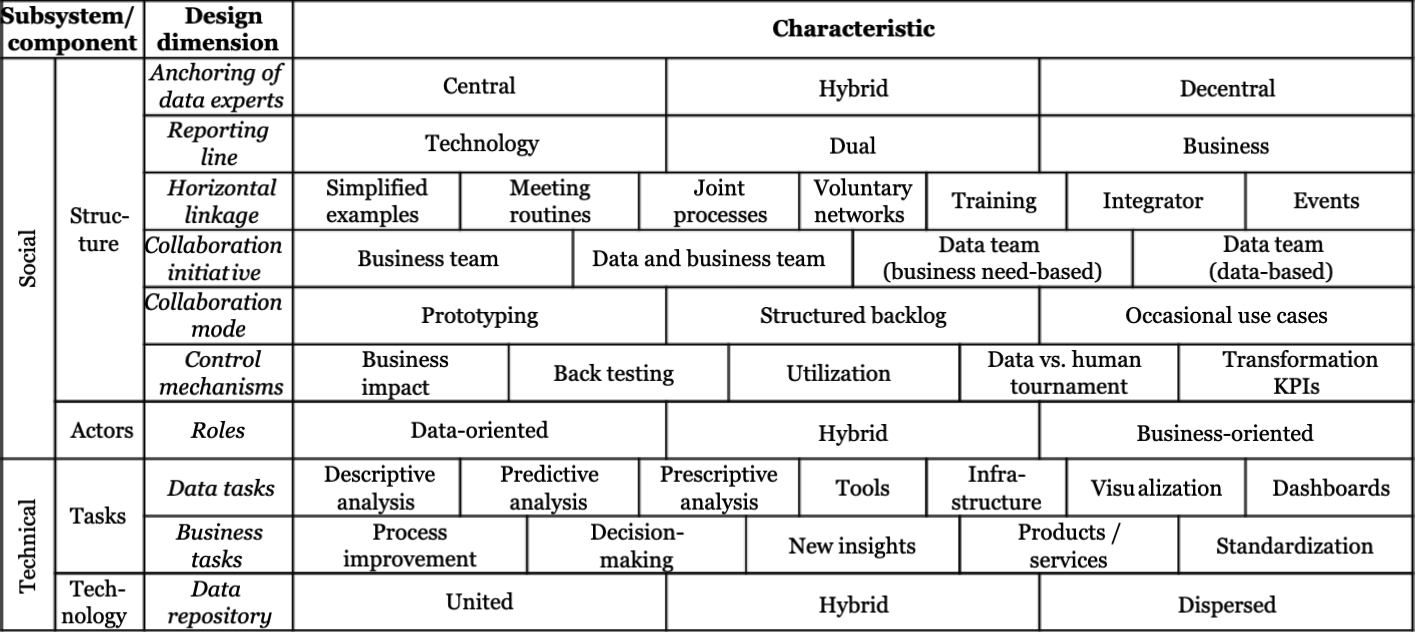
\includegraphics[width=0.95\textwidth]{graphics/DDO_design.png}
    \caption{Gestaltungsparameter einer datengesteuerten Organisation}
    \label{fig:DDOs design}
\end{figure}

Die obige Tabelle zeigt die Gestaltungsparameter organisiert nach Komponenten, Dimensionen und konkreter Charakteristika. \footcite[Vgl.][S. 5]{JanineAdinaHagen.2020}
Eine wichtige Gestaltungskomponente betrachtet die soziale Perspektive auf die Struktur und die Akteure der datengesteuerten Organisation.
Die Struktur der Organisation kann durch die Parameter \textit{Expertenorganisation, Berichtslinie, horizontale Verknüpfung, Kooperationsinitiative, Kooperationsmodus} und \textit{Kontrollmechanismus} beeinflusst werden.
Eine mögliche Ausprägung dieser Parameter umfasst z. B. zum einen dezentrale Data Science Experten, eine Berichtslinie zur Fachabteilung sowie regelmäßige Meetings und Events der Data Science Experten.
Zum anderen werden z. B. durch die Datenexperten die Zusammenarbeiten mittels strukturiertem Backlog initiiert und anhand des Geschäftsmehrwerts evaluiert.
In dieser Struktur könnten dann die Akteure z. B. hybrid, also datenorientiert sowie geschäftsorientiert gestaltet werden.
Wird die technische Perspektive betrachtet, werden dessen Komponenten der Aufgaben und Technologien durch die Parameter \textit{Datenaufgaben, Geschäftsaufgaben} und \textit{Datenrepository} bestimmt.
Beispielhaft könnte eine Organisation durch ihre Struktur und Akteure beschreibende-, prädiktive und vorhersagende Analysen erstellen, um Prozesse zu verbessern und Entscheidungen zu unterstützen.
Speicherorte für Daten und Software können z. B. hybrid für jedes Datenteam einer Fachabteilung und für den gemeinsamen Austausch mehrerer Datenteams eingerichtet werden.

\section{Experiment Evolution Model (Microsoft)}

\section{Conceptual requirements}
\section{DI / DS Integration Framework}
